\documentclass[twocolumn,linenumbers]{aastex631}

% Packages
\usepackage{microtype}  % ALWAYS!
\usepackage{amsmath}
\usepackage{amsfonts}
\usepackage{amssymb}
\usepackage{multirow}
\usepackage{tikz}
\usepackage{xcolor}
\usepackage{soul}

\definecolor{pink}{RGB}{232,132,161}
\definecolor{yellow}{RGB}{255,213,0}

\newcommand{\kc}[1]{\textcolor{yellow}{\textbf{kc: #1}} }
\newcommand\shadetext[2][]{%
  \setbox0=\hbox{{\special{pdf:literal 7 Tr }#2}}%
  \tikz[baseline=0]\path [#1] \pgfextra{\rlap{\copy0}} (0,-\dp0) rectangle (\wd0,\ht0);% 
  }
\newcommand{\ep}[1]{\shadetext[left color=blue, right color=red, middle color=lime, shading angle=45]{\textbf{e: #1}} }
% \newcommand{\ecite}[1]{\textcolor{pink}{\textbf{: #1}} }
% \newcommand{\e}[1]{\textcolor{yellow}{\textbf{: #1}} }

\newcommand{\remove}[1]{\textcolor{red}{#1}}
\newcommand{\add}[1]{\textcolor{green}{#1}}

\newcommand{\mlg}{\ensuremath{M_{\rm LG}}}
\newcommand{\mmto}{\ensuremath{M_{\rm M31}}}
\newcommand{\mmw}{\ensuremath{M_{\rm MW}}}
\newcommand{\vtan}{\ensuremath{v_\textrm{tan}}}
\newcommand{\vrad}{\ensuremath{v_\textrm{rad}}}
\newcommand{\ms}[1]{\ensuremath{M_{*{#1}}}}
\newcommand{\reflabel}[1]{\ensuremath{^{\mbox{\scriptsize{#1}}}}}
\newcommand{\scsep}{\ensuremath{\rm r_{sep}/r_{vir}}}
\newcommand{\scvel}{\ensuremath{\rm v_{rel}/v_{vir}}}

\newcommand{\paircat}{\textit{Full Pair Catalog}}
\newcommand{\Rvir}{\ensuremath{\rm R_{vir}}}
\newcommand{\Rphys}{\ensuremath{\rm R_{phys}}}
\newcommand{\Rsc}{\ensuremath{\rm R_{sc}}}
\newcommand{\rsep}{\ensuremath{\rm r_{sep}}}

\newcommand{\chambe}{\citet{Chamberlain2024}}

% Style tweaks
% \renewcommand{\twocolumngrid}{\onecolumngrid}
% \setlength{\parindent}{1.1\baselineskip}
% \sloppy\sloppypar\raggedbottom\frenchspacing

%%%%%%%%%%%%%%%%%%%%%%%%%%%%%%%%%%%%%%%%%%%%%%%%%%%%%%%%%%%%%%%%%%%%%%%%%%%%%%%%
\shorttitle{Merger Timescales in TNG100}
\shortauthors{Chamberlain et al.}

%%%%%%%%%%%%%%%%%%%%%%%%%%%%%%%%%%%%%%%%%%%%%%%%%%%%%%%%%%%%%%%%%%%%%%%%%%%%%%%%
\graphicspath{{./}{../plots/}}
% Missions
\newcommand{\project}[1]{\textsl{#1}}

% Packages / projects / programming
\newcommand{\package}[1]{\textsl{#1}}
\newcommand{\acronym}[1]{{\small{#1}}}
\newcommand{\github}{\package{GitHub}}
\newcommand{\python}{\package{Python}}
\newcommand{\astropy}{\package{Astropy}}

% Stats / probability
\newcommand{\given}{\,|\,}
\newcommand{\norm}{\mathcal{N}}
\newcommand{\pdf}{\textsl{pdf}}

% Maths
\newcommand{\dd}{\mathrm{d}}
\newcommand{\transpose}[1]{{#1}^{\mathsf{T}}}
\newcommand{\inverse}[1]{{#1}^{-1}}
\newcommand{\argmin}{\operatornamewithlimits{argmin}}
\newcommand{\mean}[1]{\left< #1 \right>}

% Non-scalar variables
\renewcommand{\vec}[1]{\ensuremath{\bs{#1}}}
\newcommand{\mat}[1]{\ensuremath{\mathbf{#1}}}

% Unit shortcuts
\newcommand{\Msun}{\ensuremath{\mathrm{M}_\odot}}
\newcommand{\Mjup}{\ensuremath{\mathrm{M}_{\mathrm{J}}}}
\newcommand{\kms}{\ensuremath{\mathrm{km}~\mathrm{s}^{-1}}}
\newcommand{\pc}{\ensuremath{\mathrm{pc}}}
\newcommand{\kpc}{\ensuremath{\mathrm{\,kpc}}}
\newcommand{\Mpc}{\ensuremath{\mathrm{Mpc}}}
\newcommand{\kmskpc}{\ensuremath{\mathrm{km}~\mathrm{s}^{-1}~\mathrm{kpc}^{-1}}}
\newcommand{\dayd}{\ensuremath{\mathrm{d}}}
\newcommand{\yr}{\ensuremath{\mathrm{yr}}}
\newcommand{\Myr}{\ensuremath{\mathrm{Myr}}}
\newcommand{\Gyr}{\ensuremath{\mathrm{\,Gyr}}}
\newcommand{\Kel}{\ensuremath{\mathrm{K}}}
\newcommand{\masyr}{\ensuremath{\mathrm{mas}~\mathrm{yr}^{-1}}}
\newcommand{\muasyr}{\ensuremath{\mu\mathrm{as}~\mathrm{yr}^{-1}}}

% Misc.
\newcommand{\bs}[1]{\boldsymbol{#1}}

% Astronomy
\newcommand{\DM}{{\rm DM}}
\newcommand{\feh}{\ensuremath{{[{\rm Fe}/{\rm H}]}}}
\newcommand{\df}{\acronym{DF}}

% TO DO
\newcommand{\todo}[1]{{\color{red} TODO: #1}}
\newcommand{\apw}[1]{{\color{blue} APW says: #1}}

% Projects
\newcommand{\gaia}{\textsl{Gaia}}
\newcommand{\gaiadr}{\textsl{Gaia}~\acronym{EDR3}}
\newcommand{\hst}{\textsl{HST}}

% Paper specific
\newcommand{\paircat}{\textit{Full Pair Catalog}}

\newcommand{\lcdm}{\ensuremath{\Lambda \rm CDM}} 
\newcommand{\sublink}{\textsc{sublink}} 
\newcommand{\subfind}{\textsc{subfind}} 

% masses - halo
\newcommand{\Mpeak}{\ensuremath{M_{\mathrm{peak}}}}
\newcommand{\Mhalo}{\ensuremath{M_{\mathrm{h}}}}
\newcommand{\MG}{\ensuremath{\rm M_{\mathrm{G}}}}
\newcommand{\mlg}{\ensuremath{M_{\rm LG}}}

% masses - stellar
\newcommand{\Ms}{\ensuremath{\rm M_{{*}}}}
\newcommand{\msam}{\ensuremath{M_{*,\mathrm{am}}}}
\newcommand{\mssim}{\ensuremath{M_{*,\mathrm{sim}}}}
\newcommand{\ms}[1]{\ensuremath{M_{*{#1}}}}

\newcommand{\vtan}{\ensuremath{v_\textrm{tan}}}
\newcommand{\vrad}{\ensuremath{v_\textrm{rad}}}
\newcommand{\reflabel}[1]{\ensuremath{^{\mbox{\scriptsize{#1}}}}}

\newcommand{\Rvir}{\ensuremath{\rm R_{vir}}}
\newcommand{\Rphys}{\ensuremath{\rm R_{phys}}}
\newcommand{\Rsc}{\ensuremath{\rm R_{sc}}}
\newcommand{\rsep}{\ensuremath{\rm r_{sep}}}

% Affiliations
\newcommand{\affuofa}{University of Arizona, 933 N. Cherry Ave,
    Tucson, AZ 85721, USA}

\newcommand{\affuofu}{Department of Astronomy, University of Utah, Salt Lake City, UT 84112, USA}

\begin{document}

\title{A Physically Motivated Framework to Compare Merger Timescales\\ of Isolated Low- and High-Mass Galaxy Pairs Across Cosmic Time
}

\author[0000-0001-8765-8670]{Katie~Chamberlain}
\affiliation{\affuofa}

\author[0000-0002-9820-1219]{Ekta~Patel}
\thanks{Hubble Fellow}\affiliation{\affuofu}


\author[0000-0003-0715-2173]{Gurtina Besla}
\affiliation{\affuofa}

\author{others}


\begin{abstract}
% Statement
Evolutionary differences between low-mass ($\rm 10^8<M_*<5\times10^9\,\Msun$) and high-mass ($\rm 5\times10^9<M_*<10^{11}\,\Msun$) galaxy pairs have been studied in detail for the last few decades, with studies finding differences in star formation rates, gas fractions, and dark matter halo profiles. 
% Problem 
Pair fraction, merger fraction, and merger rate studies of high-mass pairs have been studied extensively, both observationally and theoretically. 
However, it is unclear if using the same separation criteria to select low-mass galaxy pairs for such studies, or if using the same separation criteria at different redshifts, permits an equitable comparison between galaxies of different mass and redshift. 
% Our solution
Here, we present a physically-motivated framework by which merger timescales for high-mass and low-mass pairs can be compared equivalently 
%and converted from one system to another 
by scaling by the virial radius of the primary's FoF group halo ($r_{\mathrm{sep}}< 1 R_{\rm vir}$). 
We use the Illustris TNG100 simulation to quantify the merger timescales of isolated low-mass major pairs as a function of cosmic time, and compare to the merger timescales of similarly-selected high-mass major pairs. 
Using our framework to select pairs via a scaled separation criterion leads to equivalent merger timescales for low- and high-mass systems at redshifts $z=0-6$. 
% What are the timescales? 
Alternatively, static physical separation selections applied equivalently to all galaxy pairs at all redshifts, particularly for the closest pairs ($\rsep<150\kpc$), leads to timescales that differ by up to $\sim1\Gyr$ between low- and high-mass pairs. 
% Why it matters 
Our findings suggest that the comparison of low-mass and high-mass galaxy pair fractions, merger timescales, and merger rates is self-consistent using separation criteria that scales as a function of mass and redshift of the system. 
As a result, applying the same merger timescales to different mass systems will lead to a bias that systematically (over/under) predicts low-mass galaxy merger rates. 
\end{abstract}

%%%%%%%%%%%%%%%%%%%%%%%%%%%%%%%%%%%
\section{Introduction} \label{sec:intro}

% $z=1.5$ corresponds to snapshot \#40 in the TNG sim
% Introduce RG15, Lotz, etc.



%%% OUTLINE
\section{Methodology} \label{sec:methods}
%recap last paper and mention which data sample we narrow down to (low mass major pairs only) -- give examples of orbits
We utilize the group catalogs, produced by the \texttt{SUBFIND} algorithm~\citep{Springel2001,Dolag2009}, and the merger tree catalogs, generated by the \texttt{SUBLINK} algorithm~\citep{RG2015}, from the highest resolution run of the IllustrisTNG simulation TNG100-1 (hereafter TNG100) to study the merger timescales of galaxy pairs from $z=0-6$.
The catalogs consist of a set of 100 snapshots, ranging from $z\sim20$ (snapshot 0) to $z=0$ (snapshot 99).

Our sample consists of major (stellar mass ratio $M_{*2}/M_{*1}= 1/4 - 1$) low-mass and high-mass pairs that are isolated but physically associated.
From this sample, we will determine the fraction of pairs at each snapshot that merge before $z=0$, and track the orbits of the subhalos of each pair to study their merger timescales.

\subsection{Pair sample}
We begin with an extension of the \paircat{} described in ~\citet{Chamberlain2024}, which consists of a collection of isolated subhalo pairs at each snapshot in TNG100. 
Rather than only considering pairs for $z<4$, we will collect our base sample at each redshift in the simulation (from $z=0-\sim 27$). 
A brief version of the selection routine is transcribed here for completeness, and note that more detail and discussion of the choices for selection criteria are in Sec.~2 of~\citet{Chamberlain2024}. 

At each snapshot, low-mass and high-mass pairs are chosen by first selecting the two most massive halos (by stellar mass) from FoF groups with virial mass\footnote{We use \texttt{Group\_M\_TopHat200} from the TNG100 Group Catalogs as the FoF Group virial mass. This mass is defined to be the mass enclosed by a sphere with mean density $\Delta_c *\rho_c$, where $\Delta_c$ is the overdensity constant from~\citet{Brynorman1998} and $\rho_c$ is the critical density of the universe at the time calculated. The corresponding virial radius in TNG100 is given by \texttt{Group\_R\_TopHat200}.} 
\begin{align*}
        \mbox{\textbf{low mass:}}&\,\rm M_{G} = 8\times 10^{10}- 5\times 10^{11}\,\Msun \\ 
        \mbox{\textbf{high mass:}}&\, \rm M_{G}=1\times 10^{12}- 6.5\times10^{12}\,\Msun.
\end{align*}
Utilizing the most massive subhalos from the same FoF group ensures that the pairs are isolated from other massive nearby systems that could perturb the dynamical state of the pair. 

We require that subhalos constituting a pair meet a minimum subhalo mass criteria of 
\begin{equation*}
    \mbox{\textbf{minimum subhalo mass:}}\,
    \Mhalo > 1\times10^{9}\Msun.
\end{equation*}
at the snapshot of consideration. 
For each halo in the FoF group that passes the minimum subhalo mass criteria, we utilize the \texttt{SUBLINK} catalogs to trace their mass history~\citep{RG2015}, and find the peak halo mass of each subhalo. 

Stellar masses are then assigned to each subhalo in the FoF group using the abundance matching prescription of \citet{Moster2013}. 
The peak halo mass and current redshift are used to calculate the stellar mass of each subhalo, so that the abundance matching prescription is of the form $\ms{}=f(\Mpeak,z)$, with $z$ the redshift of consideration.

In \citet{Chamberlain2024}, the abundance matching prescription was sampled 1000 times for each subhalo to account for the spread in the Stellar Mass -- Halo Mass relation. 
However, for the purposes of the present study, we only use the stellar masses given by the median of the abundance matching relationship. 
This choice permits a roughly 1:1 monotonic relationship between stellar mass and peak halo mass, so that taking subsamples of the lowest stellar mass objects will result in a subsample with lower peak halo mass as well. % is this a good enough reason? 
Additionally, ~\cite{Chamberlain2024} found that the spread in the number of pairs selected at a given redshift is small, such that we expect the spread on the timescale analysis to be dominated by the redshift spacing of the simulation. 

Primary halos are defined as the subhalo with the highest stellar mass ($M_{*1}$) in their FoF group, and secondaries are defined as the second most massive subhalo with stellar mass $M_{*2}$. 
Our sample of major pairs then consists of all pairs of primary and secondary halos with 
\begin{align*} 
\mbox{\textbf{low mass primaries:}}&\, 10^{8}< \rm M_{*1} < 5\times10^{9} \Msun \\ 
\mbox{\textbf{high mass primaries:}}&\, 5\times 10^{9}< \rm M_{*1} < 10^{11} \Msun\\
\mbox{\textbf{stellar mass ratio:}}&\,      
    M_{*2}/M_{*1} > 1/4.
\end{align*}
A primary or secondary halo can only be a member of one single pair at a given snapshot, such that a collection of $N$ pairs consists of $N$ unique primaries and $N$ unique secondaries.

% i am removing the 10kpc component of this because I think it'd just be easier to handle those cases in the 
% Finally, we will only consider pairs that have physical separations of $\rsep>10\,\kpc$ at the snapshot of selection. 
% The physical separation cut does not vary with redshift, and is the same for both low-mass and high-mass pairs. 

The base sample of pairs used for this analysis then consists of the set of all low-mass and high-mass major pairs from each redshift of the TNG100 simulation. 


\subsection{Mergers}
% Plot \#1: Merger fraction either before or after orbits
% Note that it is very interesting that dwarf pairs in the field have high merger fractions, while the likelihood of merger is very low in more dense environments (add citation).

The primary and secondary subhalos of each pair have a `SubfindID' that is used to identify them in the \texttt{Subfind} merger tree catalogs, which contain information about every FoF group and subhalo at each redshift. 
The \texttt{SUBLINK} catalogs track subhalos from one redshift to the next, and thus enable us to track subhalos both backwards and forwards in time from any given redshift. 

We utilize the \texttt{DescendantID} field of the \texttt{SUBLINK} catalogs to determine which pairs from our base sample merge before the end of the simulation (at $z=0$) and when the merger occurs. 
The \texttt{DescendantID} field provides the `SubhaloID'\footnote{Note that the `SubhaloID' is distinct from the `SubfindID', and is unique for every subhalo in the merger trees. 
The \texttt{SUBLINK} catalogs provide the associated `SubfindID' of each subhalo.} of the subhalo's descendent in the next (or one of the following) snapshot, if it has one. 
% By following the \texttt{DescendantID}, you follow a subhalo through all of it's mergers to the `root' of the merger tree.  

A pair will be classified as a merger if the primary and secondary subhalo share the same \texttt{DescendantID} at the same redshift. 
This means that the primary and secondary subhalo will merge, producing a single descendant subhalo, by the following redshift from the simulation.
If a pair consists of a primary and secondary that never share a \texttt{DescendantID} at a given redshift, the pair is defined as a `non-merger.'

For each merging pair, we define the `merger redshift' as the redshift that immediately follows the first snapshot where the primary and secondary have the same \texttt{DescendantID}. 
For example, if the primary and secondary have different \texttt{DescendantIDs} from $z=6$ to $z=2$, but have the same \texttt{DescendantID} at $z=2$, then the merger must take place some time between $z=2$ and $z=1.9$, which is the next redshift in the simulation. 
We take $z=1.9$ to be the merger redshift. 

\subsection{Orbits} 
\begin{figure}[tb]
    \begin{center}
    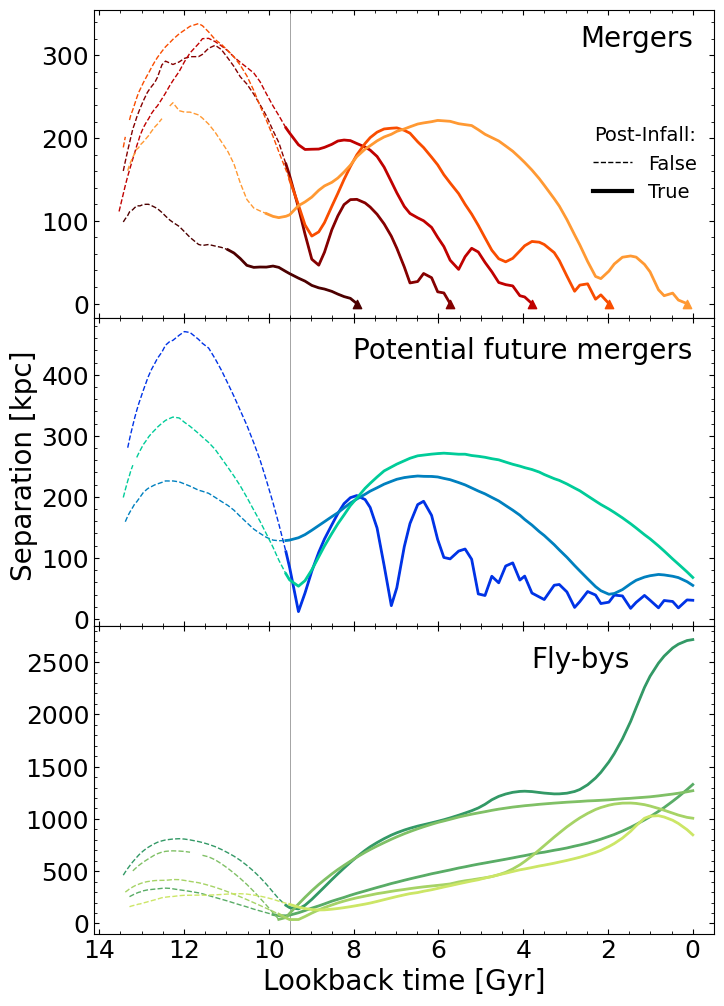
\includegraphics[width=\columnwidth]{plots/bet-on-it/5_exampleorbits.png}
    \caption{Selection of example orbits of low-mass major pairs that pass the pair selection criteria at $z=1.5$, showing the separation between the primary and secondary halo of the pair as a function of lookback time. 
    (Top) Orbits of pairs that merge before $z=0$.
    (Middle) Orbits of pairs that do not merge before $z=0$ (non-mergers), but are likely to merge if the simulation continued. 
    (Bottom) Orbits of pairs that do not merge before $z=0$ (non-mergers) and are unlikely to do so in the future $\sim2\Gyr$ (past the end of the simulation).
    Solid lines represent the post-infall parts of the orbit, while the dashed lines show the pre-infall portion of the orbit before the pairs first share a common FoF group. 
    Triangle points in the first panel show the first redshift after merger where the orbit has a separation of $0\,\kpc$.
    The vertical grey line marks $z=1.5$ at a lookback time of $9.5\,\Gyr$. 
    }
    \label{fig:example-orbits}
    \end{center}
\end{figure}

We extract orbits for all mergers and non-mergers in our base pair sample. 
An orbit for a single pair is defined to be the physical separation between the primary and secondary subhalo as a function of redshift (or lookback time). 

A given pair from the base sample at redshift $z_n$, which by definition passes all selection criteria at $z_n$, can be followed backwards and forwards in time using the \texttt{SUBLINK} merger trees.  
We track the positions of both the primary and secondary subhalo at each redshift and calculate the physical separations after accounting for the periodic boundary conditions of the simulation box.
In cases where the primary or secondary does not have a defined position at a given redshift, we set the separation at that snapshot to NaN.\footnote{If a subhalo is very small, or is passing through a more massive subhalo, and is unable to reach the density contrast required to be identified as an independent structure by the Subfind algorithm, it will not have a defined position in the Sublink catalogs. The sublink algorithm allows for subhalos to skip a single snapshot, and identifies the `skipped descendent' in the $S_{n+2}$ snapshot, so that the orbit can be evaluated before and after the skip occurs. See Sec.~3 in ~\citet{RG2015} for more details.}

In addition to the physical separation, we also calculate the scaled separation of a pair at each snapshot. We use the definition of scaled separation from~\cite{Chamberlain2024}, where the physical separation is written instead as a fraction, $p$, of the virial radius $\rsep=p\Rvir$, where $\rsep$ is the physical separation in $\kpc$, and $\Rvir$ is the virial radius of the pair's FoF group.\footnote{Where the secondary is not in the same FoF group as the primary, the virial radius used to calculate the scaled separation will remain that of the primary's FoF group, which merging secondaries will eventually re-enter prior to merger.} 
The $\Rvir$ of the pair's FoF group reasonably approximates the virial radius of a halo with a virial mass equal to the combined subhalo mass of the primary and secondary.
This ``scaled separation" is, by construction, a function of mass and redshift, which will account for the mass difference between low-mass and high-mass pairs and for halo growth over time. 

We collect the following data for each pair at each redshift where the primary and secondary are both defined: the virial mass of the primary's FoF group \texttt{Group\_M\_TopHat200}, the virial radius of the primary's FoF group \texttt{Group\_R\_TopHat200}, the physical separation (in $\kpc$), and the scaled separation (dimensionless).

\subsubsection{Defining Post-Infall}
While the orbit of a pair may be calculated at very early times, we wish to constrain our orbital analysis to only physically associated pairs, and thus will not consider the orbit of a subhalo pair before they are a part of the same FoF group. Specifically, we will consider only the ``post-infall" part of each pair's orbit. 

We define the redshift of ``first infall" as the redshift of the first snapshot where the primary and secondary have the same parent FoF halo, and post-infall is all following redshifts starting with the redshift of first infall. 

Figure~\ref{fig:example-orbits} presents a set of example orbits, which shows the wide variety of orbit-types that can be found in the TNG100 simulation for pairs that were originally selected at $z=1.5$. 
The top panel shows the orbits of 5 pairs that merge, where solid lines show the post-infall parts of the orbit, and dashed lines show the pre-infall portions of the orbit, before the secondary and primary ever share a FoF group halo. 
Even amongst galaxies of the same approximate mass and stellar mass ratio, the spread of merger timescales can be very large, with merger timescales between $\sim1-10\Gyr$ from first infall to merger. 

Some secondary subhalos can experience first infall and, after a pericentric passage, can return to such distances that they are temporarily assigned a different FoF group halo. 
Because all of our mergers occur when the subhalos are in the same FoF group, the
post-infall orbit definition is more robust for considering the full interaction timescales of merging pairs than considering the orbit only when the FoF group of the primary and secondary are the same. 
% a variety of different orbits 

The middle panel of Fig.~\ref{fig:example-orbits} (``Potential Future Mergers") shows the orbits for 3 pairs that are classified as non-mergers, since they do not merge before $z=0$, but which appear likely to merge within a few Gyr past the end of the simulation. 
These orbits can have a variety of orbital periods, and the number of pericentric passages can vary significantly. 
The two lighter blue orbits are very long period orbits with 1-2 pericenter passages in the past $10\,\Gyr$, while the darker blue orbit has a much shorter period with many close encounters throughout, and 3 close passages in just the past $2\,\Gyr$.

The bottom panel shows the orbits of "Fly-by" interactions (non-mergers) that are unlikely to merge in the near future, if ever.  
Note that we do not split our non-merger category into fly-bys and potential future mergers for any of our following analyses, and such distinctions were made only for the purposes of showing the diversity of orbits that pairs selected at the same snapshot may follow.


\subsubsection{Uniqueness of orbits}
A given pair from the \paircat{} may pass our selection criteria at many redshifts. 
Since we collect the full orbit (the separation at every redshift where the primary and secondary both exist) for each pair and each redshift, the orbits that are collected for pairs that pass our selection criteria at more than one redshift will all result in identical orbits. 
% However, we only want to keep a single instance of any given orbit in our catalog. 

To distinguish the collection of unique orbits, each pair is assigned a `pairkey' while constructing their orbit. 
The pairkey is created by concatenating the earliest SubhaloID of the primary and secondary subhalo from the Sublink catalogs, and is unique for each pair of halos. 
After each pair is assigned a unique pairkey, we save the orbit as a function of time only once for a pair that otherwise would have been double/multi-counted in our orbit catalog.

Note that a single subhalo may be a member of many different pairs, but will only have one unique orbit per unique pair.
For example, the primary of a low-mass pair selected at $z=3$ that merges before $z=2$ may be selected via our selection criteria again at $z=1$ with a new secondary companion. 
In this case, both orbits (of the original low-mass pair and the new pair which includes the remnant subhalo from the previous merger) are retained in the orbit catalog, since each orbit is unique.

Removing multiplicity decreases the raw number of orbits collected by collecting an orbit for each pair from the base sample. 
The total number of pairs (including double counting the same pair at multiple redshifts) is 71,429 for low-mass pairs, and 20,824 high-mass pairs. 
However, after removing all redundant orbits, there remain 22,213 low-mass orbits, and 3,029 high-mass orbits.

% For $n_k$ the number of pairs selected at snapshot $S_k$ via the selection criteria/from the base sample, the total number of pairs is given by
% \begin{equation*}
%     \sum_{k=0}^{99}\, n_k
% \end{equation*}
% The total number, and the total number of high-mass pairs is .
% After selecting only unique pairs, there remain 

The collection of all unique orbits constitutes our orbit sample, and is the dataset that will be used for the remainder of the paper.


\section{Pair Sample Properties}
\begin{figure}[htb]
    \begin{center}
    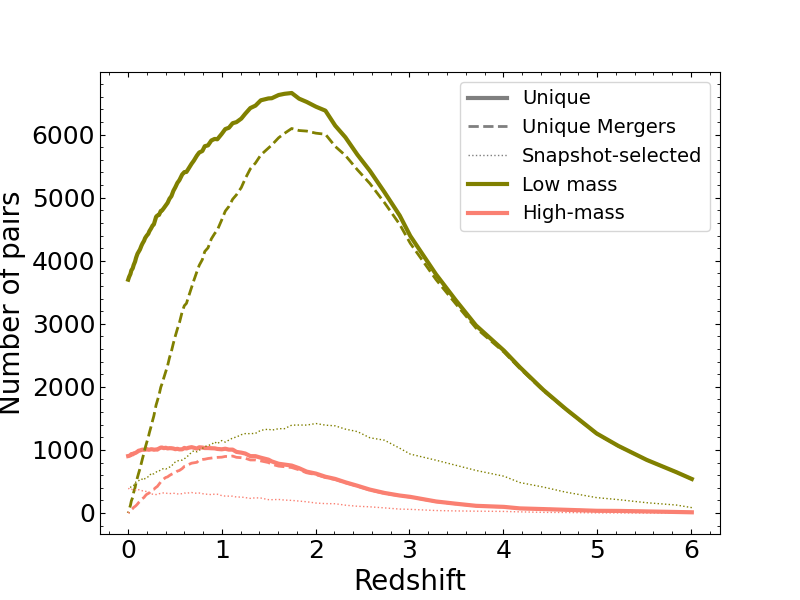
\includegraphics[width=\columnwidth]{plots/bet-on-it/6_paircount.png}
    \caption{The number of low-mass (green) and high-mass (pink) unique pairs (or distinct orbits) that are post-infall and pre-merger as a function of redshift. 
    The solid lines show the total number of orbits the are post-infall at a given redshift (including non-mergers and mergers that have yet to merge), while dashed lines show the number of post-infall orbits at a given redshift that will merge before $z=0$.
    We only count the number of orbits ``at" a given redshift if they have not merged, but have experienced first infall at a previous time (i.e. post-infall). 
    The decrease in the number of unique low-mass pairs from $z=2$ to $z=0$ is due to pairs being removed from the sample via mergers.
    }
    \label{fig:numorbits}
    \end{center}
\end{figure}

\begin{figure}[htb]
    \begin{center}
    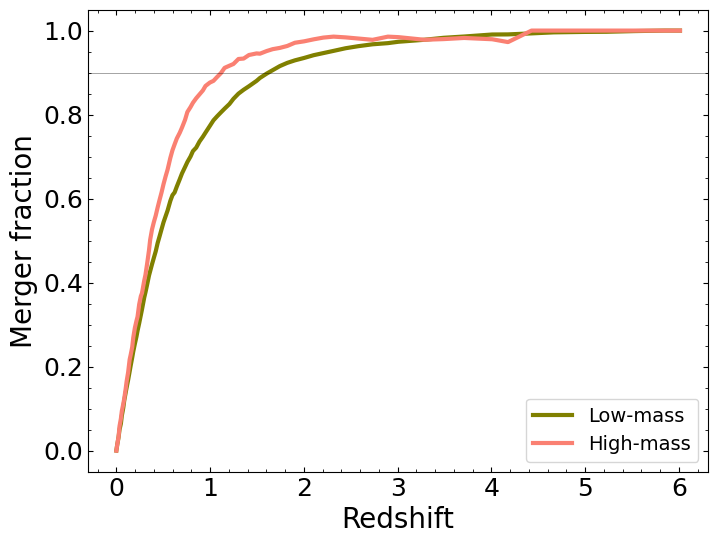
\includegraphics[width=\columnwidth]{plots/bet-on-it/6_mergerfraction.png}
    \caption{The fraction of low-mass (green) and high-mass (pink) post-infall orbits that result in a merger before z=0 as a function of redshift. 
    The horizontal line shows a merger fraction of 0.9, or 90\%. 
    High-mass pairs have merger fractions greater than 0.9 for $z>1.1$, and low-mass pairs for $z>1.6$.
    %At $z>1$, the fraction of selected pairs that merge before $z=0$ is upwards of 80\% for both low mass and high mass isolated pairs. 
    The sharp decline of the merger fraction to 0 at low redshift is a non-physical feature of the simulation ending at $z=0$.
    Only orbits with sufficiently short merger timescales will be able to merge at these redshifts.}
    \label{fig:fmerge}
    \end{center}
\end{figure}

\subsection{Number of Orbits}
We calculate the number of orbits (or orbits in progress) by selecting all orbits at a given redshift that are post-infall and either pre-merger or non-mergers.
The number of orbits that result in mergers at a later redshift are selected in the same way, excluding the non-merging orbits.
For example, the total number of orbits at $z=2$ includes the orbits of pairs that passed the selection criteria at \textit{any} redshift, provided they achieved first infall at $z\geq2$ and have a merger redshift $z<2$. 
A single pair (or equivalently, the pair's orbit) orbit may meet the conditions of being a "post-infall + pre-merger" pair for $z=0-3$, and will thus contribute to the number of orbits at all redshifts from $z=0-3$. 

Figure~\ref{fig:numorbits} shows the number of low-mass and high-mass orbits as a function of redshift from $z=0-6$. 
Low-mass orbits (green solid line) are most numerous between $z=1.25-2$, while unique high-mass pairs (pink solid line) are most numerous between $2=0-1$.
The dashed lines show the number of unique pairs that merge prior to $z=0$ for each sample. 
The number of pairs that merge decreases to 0 at $z=0$ since 
%pairs selected at $z=0$ by definition have not merged, and thus will not have the chance to, and 
many pairs that exist at low redshift will have merger timescales longer than the remaining time to the end of the simulation. 

% removed
% The thin dotted green and pink lines show the number of pairs selected at each snapshot individually, so pairs at $z=1$ that do not pass the snapshot-selection criteria at $z=2$ are not included in the number of pairs at $z=2$, but may still be counted at all snapshots where the selection criteria are met. 
% These lines are similar to the pair count lines for low-mass and high-mass pairs from Fig.~1 in~\cite{Chamberlain2024}, but only include the number of major pairs rather than the total number of pairs.

\subsection{Merger Fraction}
We calculate the merger fraction by dividing the number of merging orbits (dashed lines in Fig.~\ref{fig:numorbits}) by the number of total unique orbits (solid lines) at a given redshift. 
As before, an orbit with first infall at $z=2$ and merger at $z=1$ will be included in the merger fraction calculation for redshifts $z=1-2$.

Figure~\ref{fig:fmerge} shows the fraction of isolated pairs of low-mass (green) and high-mass (pink) pairs that merge before the end of the simulation as a function of redshift. 
At redshifts $z>2$, the merger fraction for low-mass and high-mass pairs is greater than $0.9$.
The merger fraction for both mass ranges declines to $0$ at $z=0$, due to the very low fraction of pairs at low redshift ($z<1$) that have short enough merger timescales to merge before $z=0$. At $z=0$, any remaining pairs are classified as non-mergers since they did not merge \textit{$z=0$}.

Note that the merger fraction is a measure of the fraction of isolated pairs that merge before $z=0$. 
It is not, however, a measure of the fraction of \textit{all} low-mass and high-mass pairs that will merge. 




% ###########################################################################################
% Results I
% ###########################################################################################

\section{Results: The Mass and Redshift Dependence of Merger Timescales}
We have created catalogs of unique orbits for a large sample of isolated low-mass and high-mass pairs in the TNG100 simulation.
Next, we will calculate the merger timescales, or time until merger, for all of the merging orbits in our catalog. 
In Sec.~\ref{sec:results-timevsep}, we explore how the time until merger changes as a function of the separation of the pair at a variety of redshifts, and study how the time until merger changes between the low-mass sample and high-mass sample. 
In Sec.~\ref{sec:results-timevredshift}, we investigate the median time until merger for all post-infall and pre-merger isolated pairs as a function of redshift. 
We will additionally examine the merger timescale's dependence on a variety of separation criteria. 

In the following analysis, we will utilize the orbit catalog, which consists of the unique orbits for all low-mass and high-mass major isolated pairs from the~\citet{Chamberlain2024} study. 
At a given redshift, we will include all merging pairs that are post-infall and pre-merger at that redshift in our analysis. 
However, separation criteria will also be applied to each redshift independently, so a pair that is in the $10-50\,\kpc$ bin at one redshift will not be part of the sample used at redshifts where it's separation is $>50\,\kpc$.



\begin{figure*}[htb]
    \begin{center}
    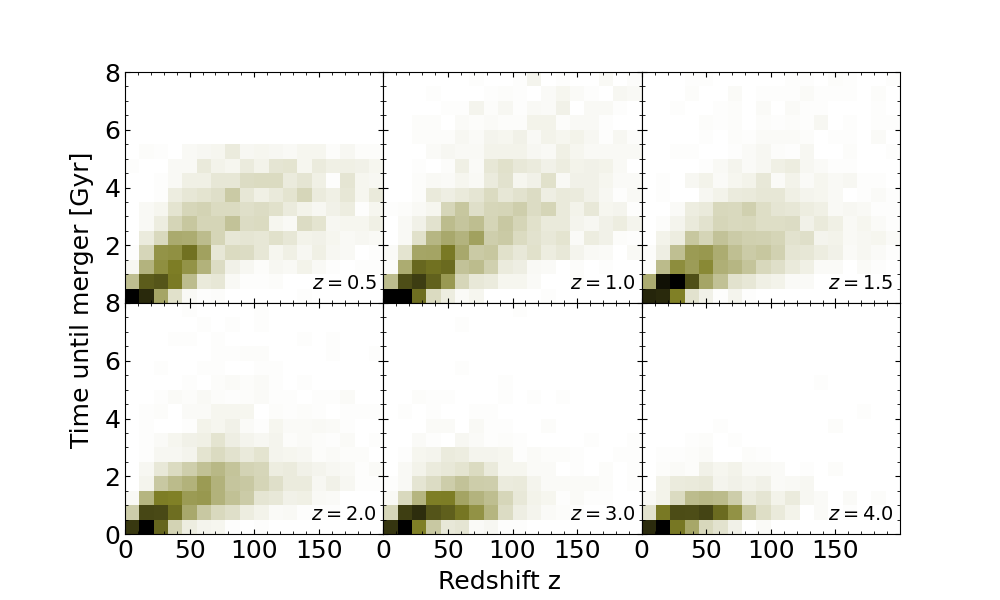
\includegraphics[width=\textwidth]{plots/bet-on-it/3_Timevsseplow-2d.png}
    \caption{\kc{Add z=5, z=6 panels. Add colorbar for percentage per panel (and add number of pairs at that redshift) Add low/high label somewhere, is the lower sep set to 10kpc?} The distribution of times until merger for low-mass pairs as a function of physical separation at $z=0.5,1,1.5,2,3,\mbox{and }4$. 
    There is a positive correlation between separation at the selected redshift and the time until merger. 
    Of orbit-selected merging pairs at $z=1$, the majority are found with separations $\rsep<100\,\kpc$, and will merge within $3-4\, \Gyr$. 
    Merger times are longer for lower redshift pairs, and the distribution of separations is larger.
    The lowest separation pairs have the shortest merger timescales.
    This plot can be used to get estimates for the merger timescale of an isolated low-mass pair at a given redshift. For example, a low-mass pair at $z=2$ with $\rsep\sim 75\,\kpc$ will merge in $0-6\,\Gyr$, with a most likely time to merger of around $2\Gyr$.
    \kc{add z=5, z=6}
    }
    \label{fig:timevssep-low}
    \end{center}
\end{figure*}

\begin{figure*}[htb]
    \begin{center}
    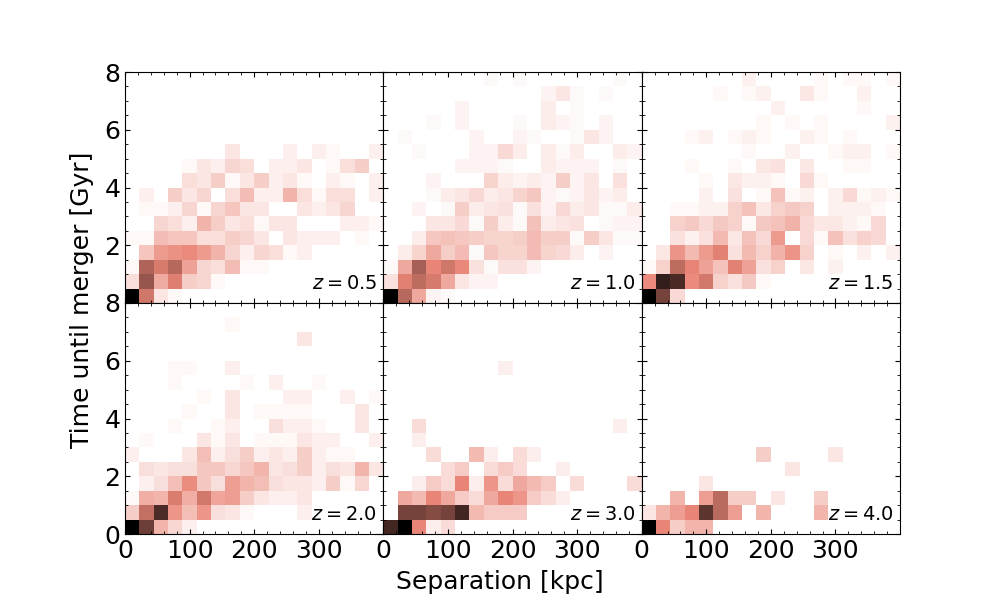
\includegraphics[width=\textwidth]{plots/bet-on-it/3_Timevssephigh-2d.png}
    \caption{\kc{Add z=5, z=6 panels. Add colorbar. Add low/high label somewhere, check the lower sep set to 10kpc?} The distribution of times until merger for high-mass pairs as a function of physical separation at $z=0.5,1,1.5,2,3,\mbox{and }4$.
    Similar to the low-mass pairs, there is a positive correlation between the separation of a merging pair at a given redshift and the time until merger, with the lowest separation pairs tending to have the shortest time until merger.
    Of orbit-selected merging pairs at $z=1$, the majority are found with separations $\rsep<200\,\kpc$, and will merge within $0-7\, \Gyr$. 
    This plot can be used to get estimates for the merger timescale of an isolated high-mass pair at a given redshift. 
    For example, a high-mass pair at $z=2$ with $\rsep\sim 150\,\kpc$ will merge in $0.5-4\,\Gyr$, with a most likely time to merger of around $1.5-2\Gyr$.
    }
    \label{fig:timevssep-high}
    \end{center}
\end{figure*}

\subsection{Separation Dependence of Merger Timescales}\label{sec:results-timevsep}
\kc{note: this might go in the appendix as additional info}
% how we calculate for this section
We calculate the time until merger as a function of separation for low-mass and high-mass pairs at a variety of redshifts from $z=0.5-6$. 
At the given redshift, we identify all merging pairs that are post-infall and pre-merger, then find the associated time difference between the given redshift and the redshift of merger for each pair.

% low mass example
For example, at $z=1.5$, there are 5,787 unique orbits that are post-infall and will merge prior to $z=0$. Of those, and 2,458 (42.47\%) have low separations between $\rsep=10-50\,\kpc$, and 2,207 of those low-separation pairs will merge in the next $2\,\Gyr$. 
A compilation of this data is available in Table~\ref{tab:timevssepvsz}, where we list the fraction of post-infall and pre-merger pairs within 3 separation bins $(10-50, 10-70, 10-100)\,\kpc$, and the fraction within each of those separation bins that merge in 4 different timescale bins $(0-1, 1-2, 2-3, 3+)\,\Gyr$, for redshifts of $z=(0.5,1,1.5,2,3,4,5,6)$.. 

As an accompanying visual aid, figures~\ref{fig:timevssep-low} and~\ref{fig:timevssep-high} show the 2D distributions of time until merger vs. separation for low-mass and high-mass pairs at redshifts $z=(0.5,1,1.5,2,3,4,5,6)$. 
Fig.~\ref{fig:timevssep-low} presents the distribution for low-mass subhalos, and shows that the time until merger for low-mass pairs is positively correlated with the separation of the pair at each redshift, but that the positive correlation is smaller at larger redshifts. 
In addition, the spread of times until merger and separations is smaller at higher redshift  than the spread at lower redshift, likely due to the size growth of halos over time. 
% could make these same plots with scaled separation, then it would presumably show roughly the same spread for each redshift. 

Likewise, fig.~\ref{fig:timevssep-high} presents the distribution for high-mass subhalos, where the trends between time until merger and separation are roughly the same. 
At each redshift, there is a positive correlation between time until merger and separation, but the spread on either of those decreases with increasing redshift. 

These figures can be used to get approximate ranges of time until merger for a pair at a given separation and for a given redshift, and are useful for seeing the difference between the relationship between time until merger and separation for low-mass and high-mass pairs. \kc{what differences?} 
% 
\begin{table*}[]
\centering
\begin{tabular}{c|c|c|c|c|c|c|c|c|c}
\hline \hline
\multirow{2}{*}{Redshift} & Separation & Total \# & \multicolumn{7}{c}{Time Until Merger} \\ \cline{4-10}
 & [kpc] &  of Orbits & $0-0.5\,\Gyr$ & $0.5-1\,\Gyr$ & $1-1.5\,\Gyr$ & $1.5-2\,\Gyr$ & $2-2.5\,\Gyr$ & $2.5-3\,\Gyr$ & $3+\,\Gyr$  \\ \hline
\multirow{6}{*}{z=1} & 10-50 &  &  &  &  &  &  &  &  \\
 & 10-75 &  &  &  &  &  &  &  &  \\
 & 10-100 &  &  &  &  &  &  &  &  \\
 & 10-150 &  &  &  &  &  &  &  & \\
 & 10-200 &  &  &  &  &  &  &  & \\
 & 10-300 &  &  &  &  &  &  &  & \\  \hline 
 \multirow{6}{*}{z=2} & 10-50 &  &  &  &  &  &  &  &  \\
 & 10-75 &  &  &  &  &  &  &  &  \\
 & 10-100 &  &  &  &  &  &  &  &  \\
 & 10-150 &  &  &  &  &  &  &  & \\
 & 10-200 &  &  &  &  &  &  &  & \\
 & 10-300 &  &  &  &  &  &  &  & \\ 
 \hline \hline
\end{tabular}
\end{table*}


\subsection{Redshift Dependence of Merger Timescales}\label{sec:results-timevredshift}
% The behavior of time until merger as a function of redshift for low-mass and high-mass pairs:
% 1 - the full sample 
% 2 - the physical and static kpc separation-selected sample
% 3 - the mass and redshift evolving scaled separation-selected sample
We study the merger timescale of low-mass and high-mass pairs as a function of redshift. 
In particular, we consider 3 different samples of the low- and high-mass systems. 
First, we will consider the orbit sample as a whole, and quantify the median merger timescale for all low- and high-mass pairs that are post-infall and pre-merger for $z=0-6$. 
We will then consider two different sets of separation criteria to create separation-selected subsamples, the first of which are physical separation criteria that are identically applied for both mass scales and all redshifts, and the second of which defines separation criteria that vary with mass and redshift.
% We ascertain the impact of the selection criteria on these subsamples of the orbit catalog ..... based on separation-selected pairs, using a set of separation criteria that we apply independently at each redshift.

Both separation-selected samples have a lower separation criteria of $10\,\kpc$, to limit the impact of subhalos becoming indistinguishable in the \texttt{SUBFIND} catalogs.
This lower separation criteria is also commonly applied to observationally-selected pairs in studies of merger fractions and merger rates (see Sec.~\ref{sec:discussion} for further detail).

Throughout, medians at each redshift are shown by solid pink and green lines, while the 1st and 3rd quartile spread on the median is shown by the shaded regions. 

\subsubsection{Full sample}
We calculate the time until merger for all post-infall and pre-merger pairs at each redshift from $z=0-6$, and quantify the median and spread on the merger timescale as a function of redshift. 
We make no selection cuts based on pair separation, and thus include the full catalog of orbits at each redshift to calculate the merger timescale (once again, provided that they are post-infall and pre-merger at the given redshift). 
Essentially, we find the median time that any physically associated isolated pair will take to merge, provided it's a merging pair to begin with. 

Figure~\ref{fig:timescales} presents the median, and 1st and 3rd quartile spread, of the time until merger for merging pairs from $z=0-6$. 
% low vs high
Low-mass merger timescales (green) and high-mass merger timescales (pink) are roughly equivalent at all redshifts. 

% redshift evolution
The median time until merger is $\sim0.5-0.7\,\Gyr$ at $z\sim6$, then rises to a peak of $2.3-2.4\,\Gyr$ at $z\sim0.6$, then decreases to 0 at $z=0$.
The abrupt decrease to 0 from $z=0.6$ to $z=0$ is an artificial rather than a true physical feature, and is caused by the lookback time of the simulation becoming shorter than the merger timescales of more and more pairs. 
The lookback time of the simulation as a function of redshift is given by the dotted black line on the left of Fig.~\ref{fig:timescales}.
At $z=0$, the number of pairs that will merge is 0, since we cannot track the orbits of the subhalos into the future.

In addition, we show 
\begin{equation}
\frac{2}{5}*H(z)^{-1}
\end{equation}
given the Hubble parameter $H(z)$ as the dashed black line that sits above the median time until merger.
We also show the age of the simulation as a function of redshift (dashed grey).
% rest of stuff to talk about with this plot is discussion (i think) like what does this imply about the merger timescales of low vs high mass pairs? 

\subsubsection{Separation Criteria: Static \& Physical }
The first set of separation criteria will select only pairs at a given redshift that have separations greater than $10\,\kpc$ and less than $[50, 70, 100, 150, 200, \mbox{and }300]\kpc$. 
These separation criteria do not vary as a function of time or mass, and are thus applied equivalently to the low-mass and high-mass samples. 
This set of static physical separation criteria produces 6 subsamples of merging orbits that are post-infall. 

Note that an orbit in the separation bin $10-50\,\kpc$ at $z=2$ will not necessarily be in that same bin at other redshifts. 
Rather, the separation criteria select pairs with separations in the given separation bin independently at each redshift. 

% figure description 
The top panel of Fig.~\ref{fig:timescales-sep} shows the time until merger versus redshift for low-mass (green) and high-mass (pink) orbits that have separations less than the separation listed above each plot.  
% redshift evolution of each subsample
We first note that the evolution of the time until merger is approximately the same for each separation-selected subsample, with a peak time at redshift $z\sim0.5$ present for all subsamples, and a rapid decline of the median time until merger at $z=0-0.5$. 
These traits were also present in Fig.~\ref{fig:timescales} where the median time until merger was computed for the entire sample, without a selection-criterion.
As the selection-criteria gets larger and larger, the subsample will contain more and more of the full sample, eventually reconstructing the full sample plot with a large enough separation selection.

% low mass vs high mass
There is an offset between the median times for low-mass and high-mass pairs for each of the subsamples with maximum separations of $[50, 70, \mbox{and } 100]\,\kpc$. 
The difference in the median time until merger is up to $0.8\,\Gyr$ longer for low-mass pairs than high-mass pairs at the same redshift. 
The offset between the low-mass and high-mass merger times decreases for large enough physical separation criteria. 
In the rightmost top panel, the median merger times overlap almost identically for $z=0-0.5$ and $z>1.5$. 

% impact of the separation criteria
The median time until merger for pairs selected in smaller separation bins (such as $10-50\,\kpc$ and $10-70\,\kpc$) is lower at all redshifts for both low-mass and high mass pairs. 
This follows directly from Sec.~\ref{sec:results-timevsep}, where we found that the time until merger is positively correlated with increasing separation for all pairs. 
Thus, including more and more larger-separation systems in our merger time calculation will tend to increase the median time until merger. 

\subsubsection{Separation Criteria: Scaled Separation}
The second set of selection criteria will select pairs at a given redshift in 6 different scaled separation bins, where the scaled separation is written as a fraction of the virial radius of the pair's FoF group, $\Rvir$ (see Sec.~\ref{sec:methods} for more details). 
The scaled separation-selected pairs have separations greater than $10\,\kpc$ and less than $<[0.25, 0.5, 1, 1.5, 2, 2.5]\,\Rvir$. 

A scaled separation criterion scales with both redshift and mass (since the virial radius scales with redshift and mass), and produces 6 subsamples of merging orbits that are post-infall.
As mentioned in \chambe{}, the median virial radius for low-mass FoF groups at $z=[0,1,2,3,4]$ is approximately $[134, 85, 59, 43, 33]\,\kpc$, and for high-mass FoF groups is approximately $[348, 206, 134, 97, 76]\,\kpc$.
Thus, choosing a scaled separation cut of $<1\,\Rvir$ at $z=1$ will select high-mass pairs with separations $\lesssim205\,\kpc$ and low-mass pairs with separations $\lesssim85\,\kpc$.

As in the previous section, the selection criteria are applied at each redshift independently. 
This means that the time until merger of a pair at a given redshift will only be included in the calculation of the median merger time if its separation is within the given separation bin at that redshift. 

% figure description 
The bottom panel of Fig.~\ref{fig:timescales-sep} shows the median time until merger versus redshift for low-mass (green) and high-mass (pink) systems with scaled separations less than those listed above each plot. 
In the panel on the left, only pairs with a separation between $10\,\kpc-0.25\,\Rvir$ are utilized for the calculation. 
We find that the median time until merger at $z=1$ is XX..XX for each scaled separation cut respectively, for both low-mass and high-mass samples.

% redshift evolution of each subsample
Similar to the static physical separation-selected subsamples in the top panel, the median time until merger starts off small at $z>4$, then increases to a peak around $z\sim0.5$, before quickly decreasing to 0 at $z=0$. 
This behavior also mimics that of the full sample. 

% impact of the separation criteria
Additionally, the median time until merger at a given redshift increases for separation criteria that include a larger fraction of the virial radius, and thus larger separation pairs. 
This again matches the behaviour of the static physical separation criteria shown in the top panel.

% low mass vs high mass
However, quite unlike the subsamples in the top panels, the scaled separation-selected subsamples yield nearly identical median merger timescales for low-mass and high-mass pairs at all redshifts, regardless of what fraction of the virial radius is selected. 


% ###########################################################################################
% Results II 
% ###########################################################################################




\begin{figure}[htb]
    \centering
    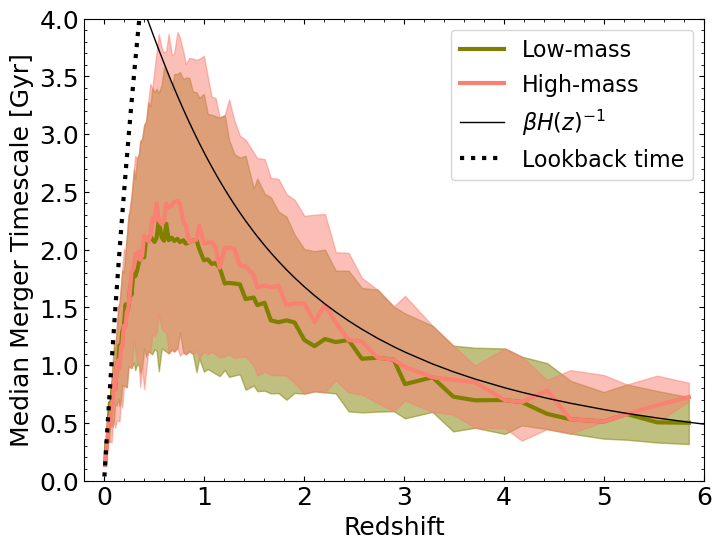
\includegraphics[width=\columnwidth]{plots/bet-on-it/8_timescale.png}
    \caption{The median time until merger as a function of redshift for low-mass (green) and high-mass (pink) pairs. Shaded regions represent the 1st and 3rd quartile spread on the median. Pairs at each redshift are selected if they have experienced first infall and are pre-merger. 
    % 
    The black dashed line shows a fraction of the Hubble time as a function of redshift, which bounds the median time until merger from $z=6$ to $z\sim0.5-0.75$.
    The dotted black line shows the time to $z=0$ (the lookback time) as a function of redshift, which sets the upper bound for the time until merger that a merging pair can have. 
    The median time until merger is similar for low-mass and high-mass pairs, and rises from $z=6$ to a peak at $z\sim0.75$, then decreases to $z=0$.}
    \label{fig:timescales}
\end{figure}

\begin{figure*}[htb]
    \centering
    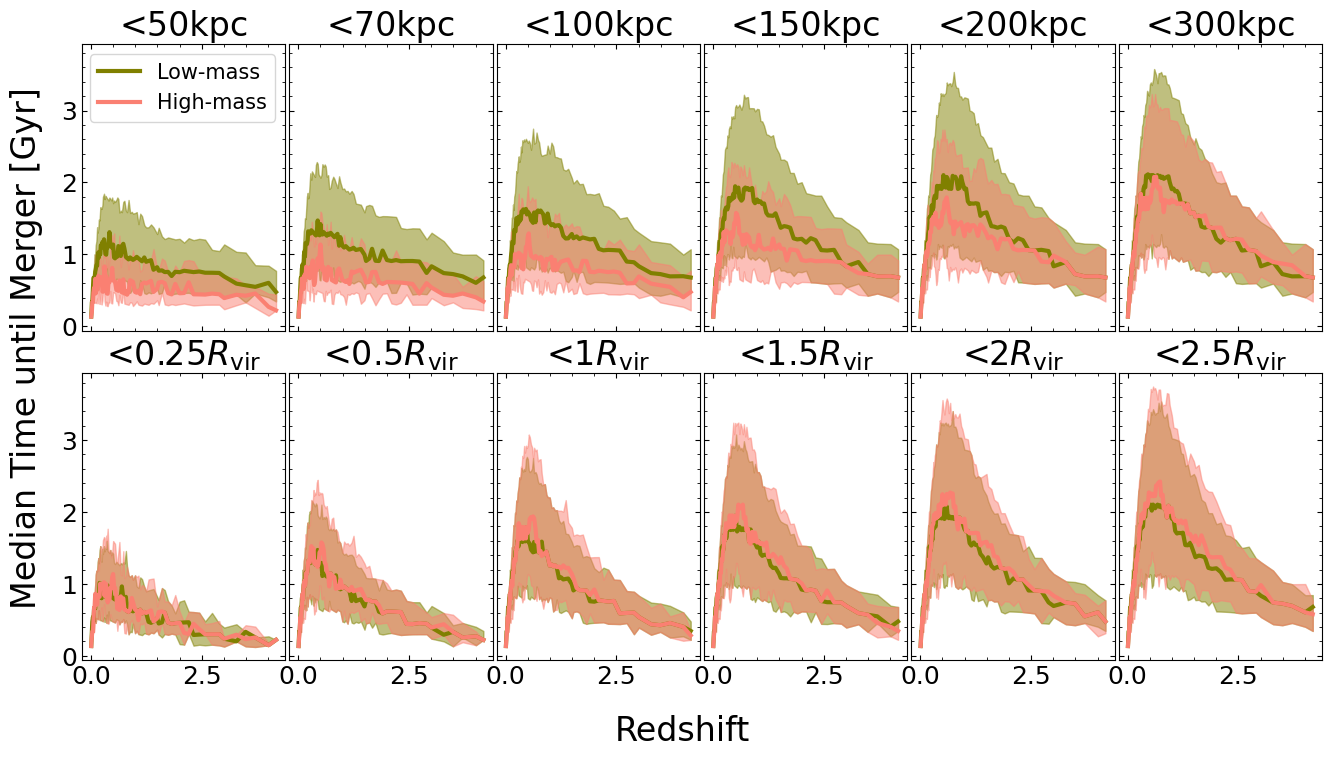
\includegraphics[width=\textwidth]{plots/bet-on-it/3_time_til_merger.png}
    \caption{(Top) The median time until merger as a function of redshift for low-mass (green) and high-mass (pink) pairs with 3D physical separations greater than $10\,\kpc$ and less than $(50,70,100,150,200,\mbox{and }300)\,\kpc$ from left to right. 
    (Bottom) The median time until merger as a function of redshift for pairs with physical separations greater than $10\,\kpc$ and less than $(0.25, 0.5, 1, 1.5, 2,\mbox{and }2.5)\,\Rvir$ from left to right. 
    % 
    The time until merger increases from $z=4$ to $z\sim0.5-0.75$, at which point the time until merger decreases to zero since all low redshift mergers must have short merger timescales to merge before the end of the simulation at $z=0$. 
    }
    \label{fig:timescales-sep}
\end{figure*}


\section{Discussion} \label{sec:discussion}

\subsection{About the number of pairs}
Can we say anything about the REASON the unique pairs decreases at low z? Does this plot mean that it's only because things merge and so we lose them? And not that it's driven by mass-accretion thing? I think so.

Need to be careful about phrasing since we didn't actually quantify the number of pairs that leave the sample due to having too large of masses at later snapshots. 

\subsection{About the merger fraction}
Were low-mass pairs expected to have such a high merger rate in isolated environs? 
How do these merger fractions compare to other literature results? 
If we can make comparisons, discuss the differences. 
If we cannot make comparisons, explain why our study is done in a way that makes for comparisons unfair/undoable .

\subsection{Results}

Why did we pick the separation cuts that we did? (motivated already in Chambe+ 2024, restate here about close pair definitions from lit.)

For a given static separation selection (particularly <50, <70, and <100), the merger timescales of low-mass and high-mass systems disagree by ~0.5\Gyr at almost all redshifts.

Scaled separation criteria are akin to picking the same fraction of the total volume of a FoF group, regardless of what redshift it is at, not what mass it has. 


\subsection{What does it mean that the Time until Merge plot has the function form that it does?}
Upper bounds of the hubble time and the lookback time as functions of z.

maybe a point: 
For things that don't merge, what's... going on? 



% \subsection{Merger Rates for Dwarf Pairs}
% % - What combination of values best reproduces the merger fraction acquired from the sims?
% % Do you need the scale of merger probability as in Ventou to get the match?
% % Vicente & Casteels 2014 comparison (pair fractions plot)
% \subsection{Pairs of Dwarfs That Do Not Merge}
% % can talk about the unmerged fraction merger rates here
% \subsection{Choosing Samples at Lower and Higher Redshift}
% % can also compare to samples to merger fractions and merger rates chosen at z=1 and z=2 (plots you have already)
% \subsection{Comparing with Merger Rates for Massive Galaxy Pairs}
% % compare to massive pairs in both obs window and merger rate
% % compare back to the assumption of isolation


\section{Summary and Conclusions}
% what we did and how


% set of conclusions from results
Our main findings are as follows: 
\begin{itemize}
    \item for a given separation (such as 100kpc), high-mass pairs have shorter merger timescales than low-mass pairs. 
    \item the median time until merger for the full sample of low and high-mass pairs increases as $\sim(1+z)^{-1}$ from $z=6$ to $z\sim0.75$. it then decreases to 0 at low redshifts, with an upper bound set by the time remaining in the simulation before $z=0$. The decrease in the merger time at low redshifts is artificial and not representative of the true merger timescales that pairs at $z=0$ will have.
    \item separation criteria that include larger separations will increase the median time until merger.
    \item static physical separation-selected subsamples of low- and high-mass pairs have different median merger timescales.
    \item scaled separation-selected subsamples yield nearly identical median merger timescales for low-mass and high-mass pairs at all redshifts. 
\end{itemize}

% set of conclusions for discussion
- We find that the merger timescale of low-mass or high-mass merging pairs is sensitive to the selection criteria that are used to define the pair sample.\\

- We recommend that future studies that seek to compare or compute pair fractions, merger fractions, merger timescales, or merger rates, define selected pair samples using separation criteria that evolve with redshift and mass. 






% ** 
% \appendix
% adfadfa








\bibliography{refs}{}
\bibliographystyle{aasjournal}

\end{document}

